% \iffalse
\let\negmedspace\undefined
\let\negthickspace\undefined
\documentclass[journal,12pt,twocolumn]{IEEEtran}
\usepackage{cite}
\usepackage{amsmath,amssymb,amsfonts,amsthm}
\usepackage{algorithmic}
\usepackage{graphicx}
\usepackage{textcomp}
\usepackage{xcolor}
\usepackage{txfonts}
\usepackage{listings}
\usepackage{enumitem}
\usepackage{mathtools}
\usepackage{gensymb}
\usepackage{comment}
\usepackage[breaklinks=true]{hyperref}
\usepackage{tkz-euclide}
\usepackage{listings}
\usepackage{gvv}
\def\inputGnumericTable{}
\usepackage[latin1]{inputenc}
\usepackage{color}
\usepackage{array}
\usepackage{longtable}
\usepackage{calc}
\usepackage{multirow}
\usepackage{hhline}
\usepackage{ifthen}
\usepackage{lscape}

\newtheorem{theorem}{Theorem}[section]
\newtheorem{problem}{Problem}
\newtheorem{proposition}{Proposition}[section]
\newtheorem{lemma}{Lemma}[section]
\newtheorem{corollary}[theorem]{Corollary}
\newtheorem{example}{Example}[section]
\newtheorem{definition}[problem]{Definition}
\newcommand{\BEQA}{\begin{eqnarray}}
\newcommand{\EEQA}{\end{eqnarray}}
\newcommand{\define}{\stackrel{\triangle}{=}}
\theoremstyle{remark}
\newtheorem{rem}{Remark}
\begin{document}

\bibliographystyle{IEEEtran}
\vspace{3cm}

\title{NCERT Discrete - 11.9.3.30}
\author{EE23BTECH11007 - Aneesh Kadiyala$^{*}$% <-this % stops a space
}
\maketitle
\newpage
\bigskip

\renewcommand{\thefigure}{\theenumi}
\renewcommand{\thetable}{\theenumi}
%fi

\vspace{3cm}
\textbf{Question 11.9.3.30:} The number of bacteria in a certain culture doubles every hour. If there were 30 bacteria present in the culture originally, how many bacteria will be present at the end of $2^{nd}$ hour $4^{th}$ hour and $n^{th}$ hour?
\\
\solution

\begin{table}[h!]
    \centering
    \caption{Input Parameters}
    \label{tab:1}
    \begin{tabular}{ | c | c | c | }
        \hline
        Parameter & In terms of x(n) & Value \\
        \hline
        Initial number of bacteria ($a_0$) & x(0) & 30 \\
        &&\\
        Ratio of bacteria at the end of the & & \\
        hour to the start of the hour ($r$) & $x(n)/x(n - 1)$ & 2 \\
        \hline
    \end{tabular}
\end{table}


\begin{enumerate}
\item
Let number of bacteria initially be $a_0$ = 30
\\
Let number of bacteria at the end of $n^{th}$ hour be $a_n$.
\\
Since number of bacteria doubles every hour, \[a_n = 2a_{n - 1}\]
\[a_n = 2(2a_{n - 2})\]
\[\dots\]
\[a_n = 2^na_0 = 2^n(30)\]
$\implies a_2 = 2^2(30) = 120$ and $a_4 = 2^4(30) = 480$
\\

Therefore, number of bacteria at the end of the $2^{nd}$ hour is 120, $4^{th}$ hour is 480, and $n^{th}$ hour is $30(2^n)$.

\item \textbf{Finding $x(n)$}

The series is a geometric progression.
\[x(n) = x(0) (r^{n})\]
where $r$ is the common ratio.\\
It is given that $x(0) = 30$, $r = 2$ (see table \ref{tab:1}).
\[\implies x(n) = 30(2^n)(u(n))\]
as $x(n) = 0 \forall n < 0$.

\begin{figure}[h!]
    \centering
    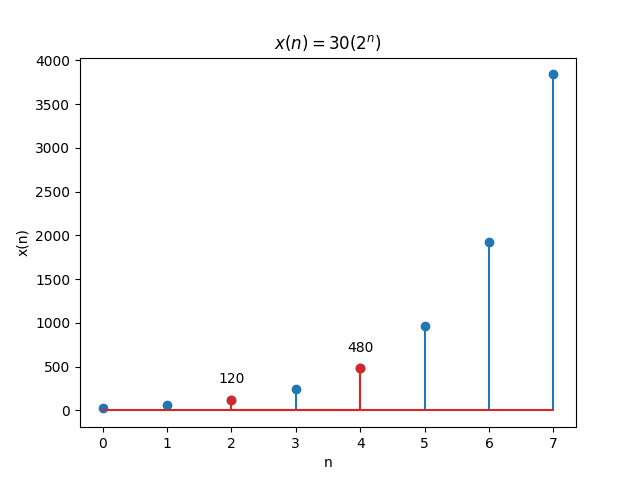
\includegraphics[width=\columnwidth]{figs/11_9_3_30.png}
\end{figure}


\item \textbf{Z-transform of $x(n)$}

Let Z-transform of $x(n)$ be $X(z)$.
\[X(z) = \sum_{n = -\infty}^{\infty} x(n)u(n)z^{-n}\]
\[X(z) = \sum_{n = 0}^{\infty} (30)(2^n)(z^{-n})\]
\[X(z) = 30\lim_{n\to\infty}\sum_{i = 0}^{n}(\frac{2}{z})^i\]

\begin{enumerate}
\item If $|z| > 2$:
\[X(z) = \frac{30}{1 - \frac{2}{z}}\]
\[X(z) = \frac{30z}{z - 2}\]

\item If $|z| \le 2$:
\[X(z) \to \infty\]

\end{enumerate}

\[\implies X(z) = \frac{30z}{z - 2} \forall |z| > 2\]

\end{enumerate}
\end{document}